\chapter{Related Work}
\label{chap:relatedwork}

\section{3D Style Transfer}

The initial objective was to explore the possibility of style transfer on 3D avatars, leading to the relatively new field of 3D style transfer in computer vision. 3D neural stylization or style transfer refers to applying neural stylization techniques to modify the visual appearance and aesthetic characteristics of pre-existing 3D digital representations \citep{Chen.2023}. To fuse 3D representation with a new style, two key factors must be considered: 3D content preservation and style transformation. In the context of 3D avatars, geometry represents the shape of the avatar, while texture represents its color. Thus, 3D avatar style transfer can be divided into two main categories: geometry-based style transfer and texture-based style transfer. Geometry-based style transfer modifies the shape of the 3D avatar, whereas texture-based style transfer alters the color of the 3D avatar. Successful style transfer on 3D avatars requires considering both the geometry and texture of the input avatar, as well as the style guidance, which can be provided as a text prompt \citep{Nguyen-Phuoc.2023, Zhang.2023, Mendiratta.2023} or a reference image \citep{Han.2021, Abdal.2023, Zhang.2024, Jaganathan.2024}. 

Some works extend image-to-image style transfer networks to directly stylize 3D objects \citep{Kang.2023}. Others leverage 2D priors to guide 3D stylization results in various representations, such as point clouds \citep{Cao.2020, Segu.2020, Luo.2021}, meshes \citep{Yin.2021, Nguyen-Phuoc.2023, Kang.2023, Yang.2023}, and implicit functions like neural radiance fields \citep{Haque.2023, Kamata.2023, Patashnik.2024}, and more recently, Gaussian Splatting \citep{Wang.2024, Liu.2024, Wu.2024, Chen.2024, Jaganathan.2024}. Many of these methods are too complex for the specific goal of stylizing a 3D avatar using multi-view images. However, several works have inspired this thesis, providing valuable insights into 3D style transfer on head avatars and a potential workflow for multi-view image style transfer.

\section{Exemplar-based 3D Portrait Stylization}
\textcite{Han.2021} propose a pipeline to generate a stylized 3D human face model with exaggerated geometry and texture transferred from a 2D cartoon image. The authors introduce a two-stage approach that disentangles the geometric and texture domains. In the first stage, the method generates a coarse 3D face stylized geometry from a real facial photo and a 2D caricature image as the style reference. This is achieved by using their multi-modal landmark translation network to map all 68 facial landmarks of the style image and the real photo, enabling the creation of a coarse global shape of the 3D face model for a deformation network using a differentiable rasterizer such as SoftRas \citep{Liu.2019}. 

In the second stage, the method focuses on performing artistic style transfer on the canonical texture using STROTSS \citep{Kolkin.2019}, while keeping the geometry fixed. A differentiable renderer is employed to render the textured model into different views and optimize the texture through a multi-view framework. The pipeline also incorporates a novel multi-view loss function to preserve the identity of the person in the real photo. As a result, it can perform both semantic and artistic style transfer through mesh deformation and texture editing. However, the pipeline is limited to a single style image and a single real photo. Upon accessing the implementation, it was observed that the pipeline functions effectively only in a very specific setting, as demonstrated in their example, and requires significant manual intervention. Figure \ref{fig:stross_texture_style} shows the application of the example style images to Photodome images. Despite the pipeline's capability to learn styles from a large dataset of style images and preprocess these images, only two compatible style images are provided.

\begin{figure}
    \centering
    \begin{subfigure}{0.22\linewidth}
        
\includegraphics[width=\textwidth]{Figures/white.png}
        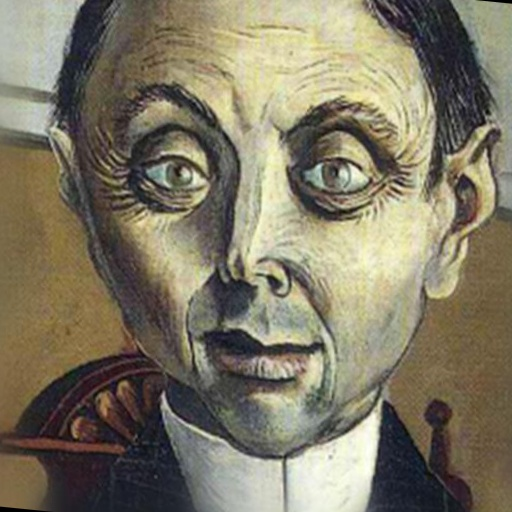
\includegraphics[width=\textwidth]{Figures/failed/stross/textures/00016_style.jpg}
        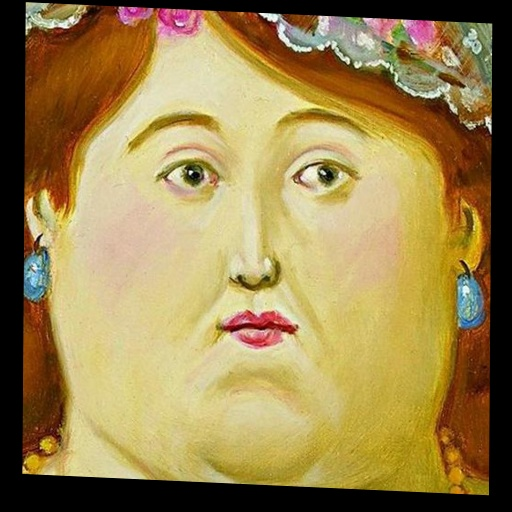
\includegraphics[width=\textwidth]{Figures/failed/stross/textures/00059_style.jpg}
	\end{subfigure}
    \begin{subfigure}{0.22\linewidth}
        
\includegraphics[width=\textwidth]{Figures/failed/stross/textures/masked/masked_head_8-8-5-1_123851_791.png}
        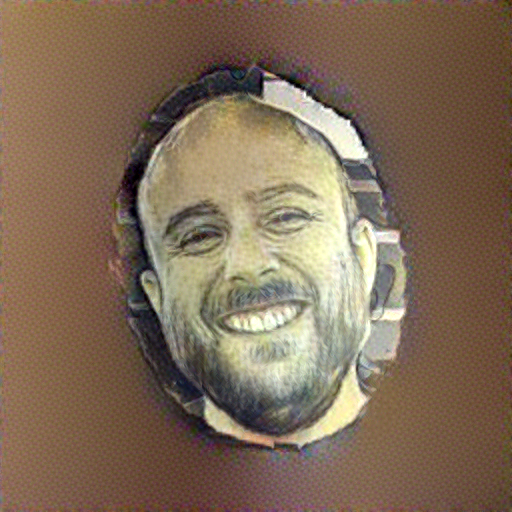
\includegraphics[width=\textwidth]{Figures/failed/stross/textures/16/stylized_view_8-8-5-1_123851_791.png}
        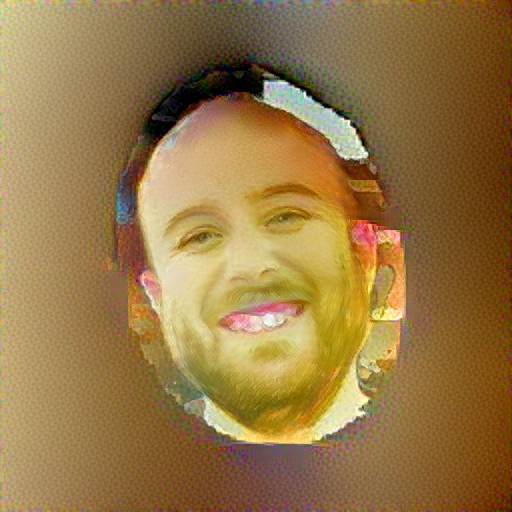
\includegraphics[width=\textwidth]{Figures/failed/stross/textures/59/stylized_view_8-8-5-1_123851_791.png}
	\end{subfigure}
    \begin{subfigure}{0.22\linewidth}
        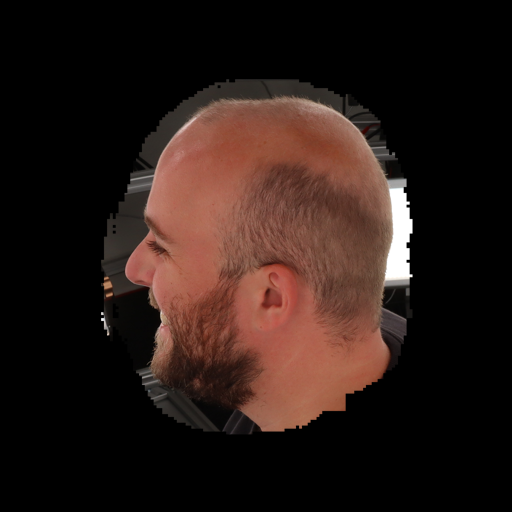
\includegraphics[width=\textwidth]{Figures/failed/stross/textures/masked/masked_head_8-5-3-2_123851_842.png}
        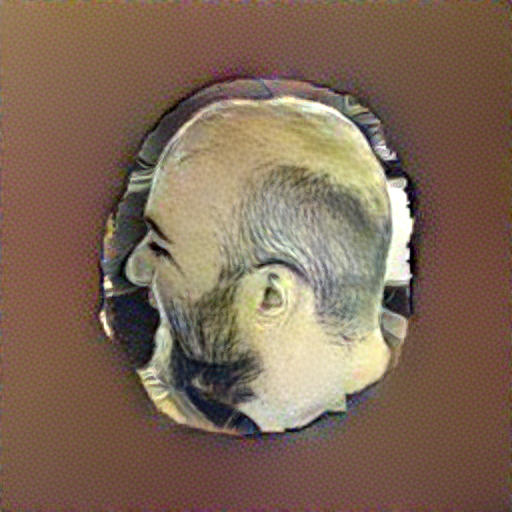
\includegraphics[width=\textwidth]{Figures/failed/stross/textures/16/stylized_view_8-5-3-2_123851_842.png}
        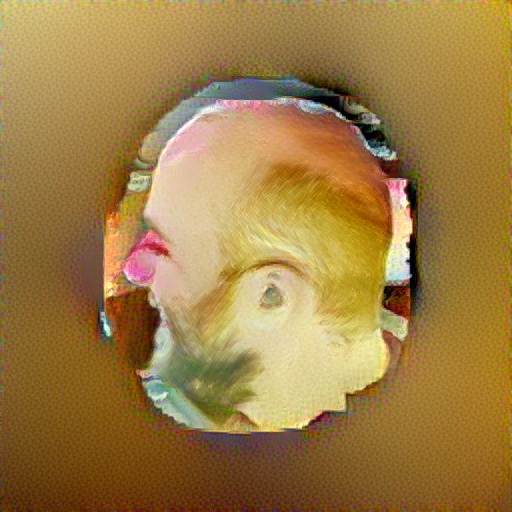
\includegraphics[width=\textwidth]{Figures/failed/stross/textures/59/stylized_view_8-5-3-2_123851_842.png}
	\end{subfigure}
    \begin{subfigure}{0.22\linewidth}
        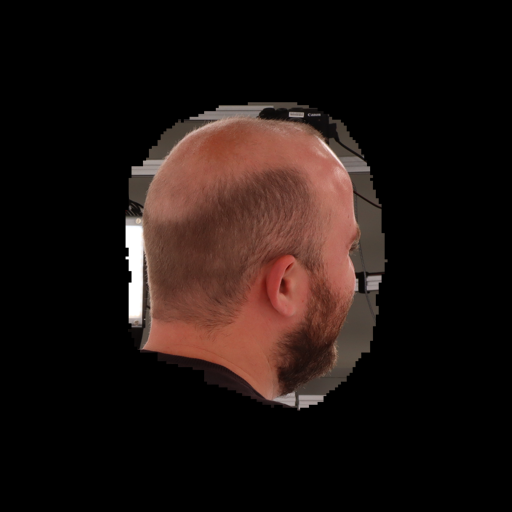
\includegraphics[width=\textwidth]{Figures/failed/stross/textures/masked/masked_head_8-C-5-1_123851_737.png}
        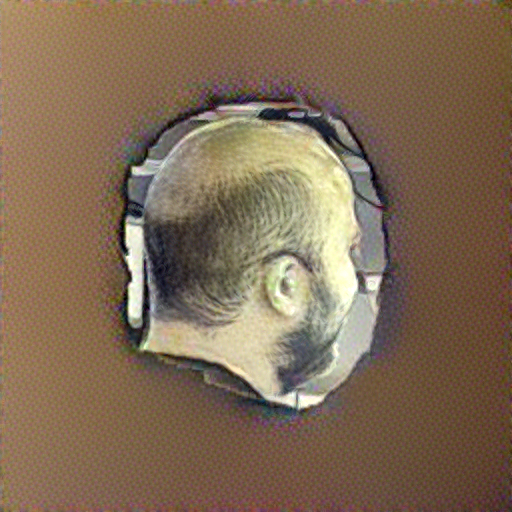
\includegraphics[width=\textwidth]{Figures/failed/stross/textures/16/stylized_view_8-C-5-1_123851_737.png}
        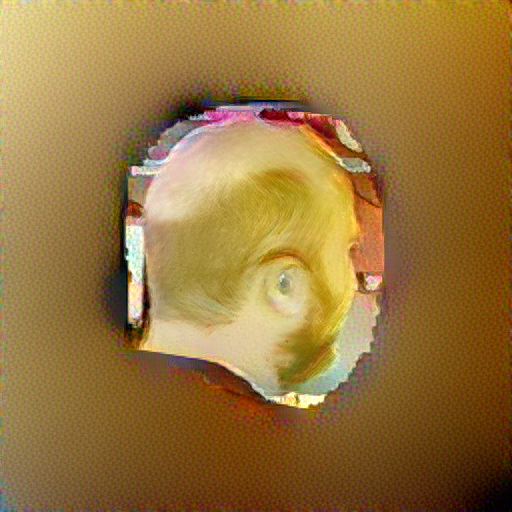
\includegraphics[width=\textwidth]{Figures/failed/stross/textures/59/stylized_view_8-C-5-1_123851_737.png}
	\end{subfigure}
    \caption{Experimentation of STROTSS pipeline with various style images applied to the masked Photodome images. The effect of landmarks translation between the style image and the Photodome images is visible in the stylized images even though it can be inaccurate in certain regions resulting in inconsistencies across views.}
    \label{fig:stross_texture_style}

\end{figure}

Furthermore, the pipeline does not provide an end-to-end solution, making it difficult to reproduce the results or adapt it for this thesis. For experimentation purposes in initial research, their style transfer pipeline was used with the Photodome dataset but without their deformation and reconstruction pipeline. Instead, a canonical 3D avatar was built using photogrammetric reconstruction, and the stylized images were remapped to its UV coordinates. The results are shown in Figure \ref{fig:stross_texture_fit}.

\begin{figure}
    \centering
    \begin{subfigure}{0.18\linewidth}
        
\includegraphics[width=\textwidth]{Figures/failed/stross/3d/snapshot09.png}
        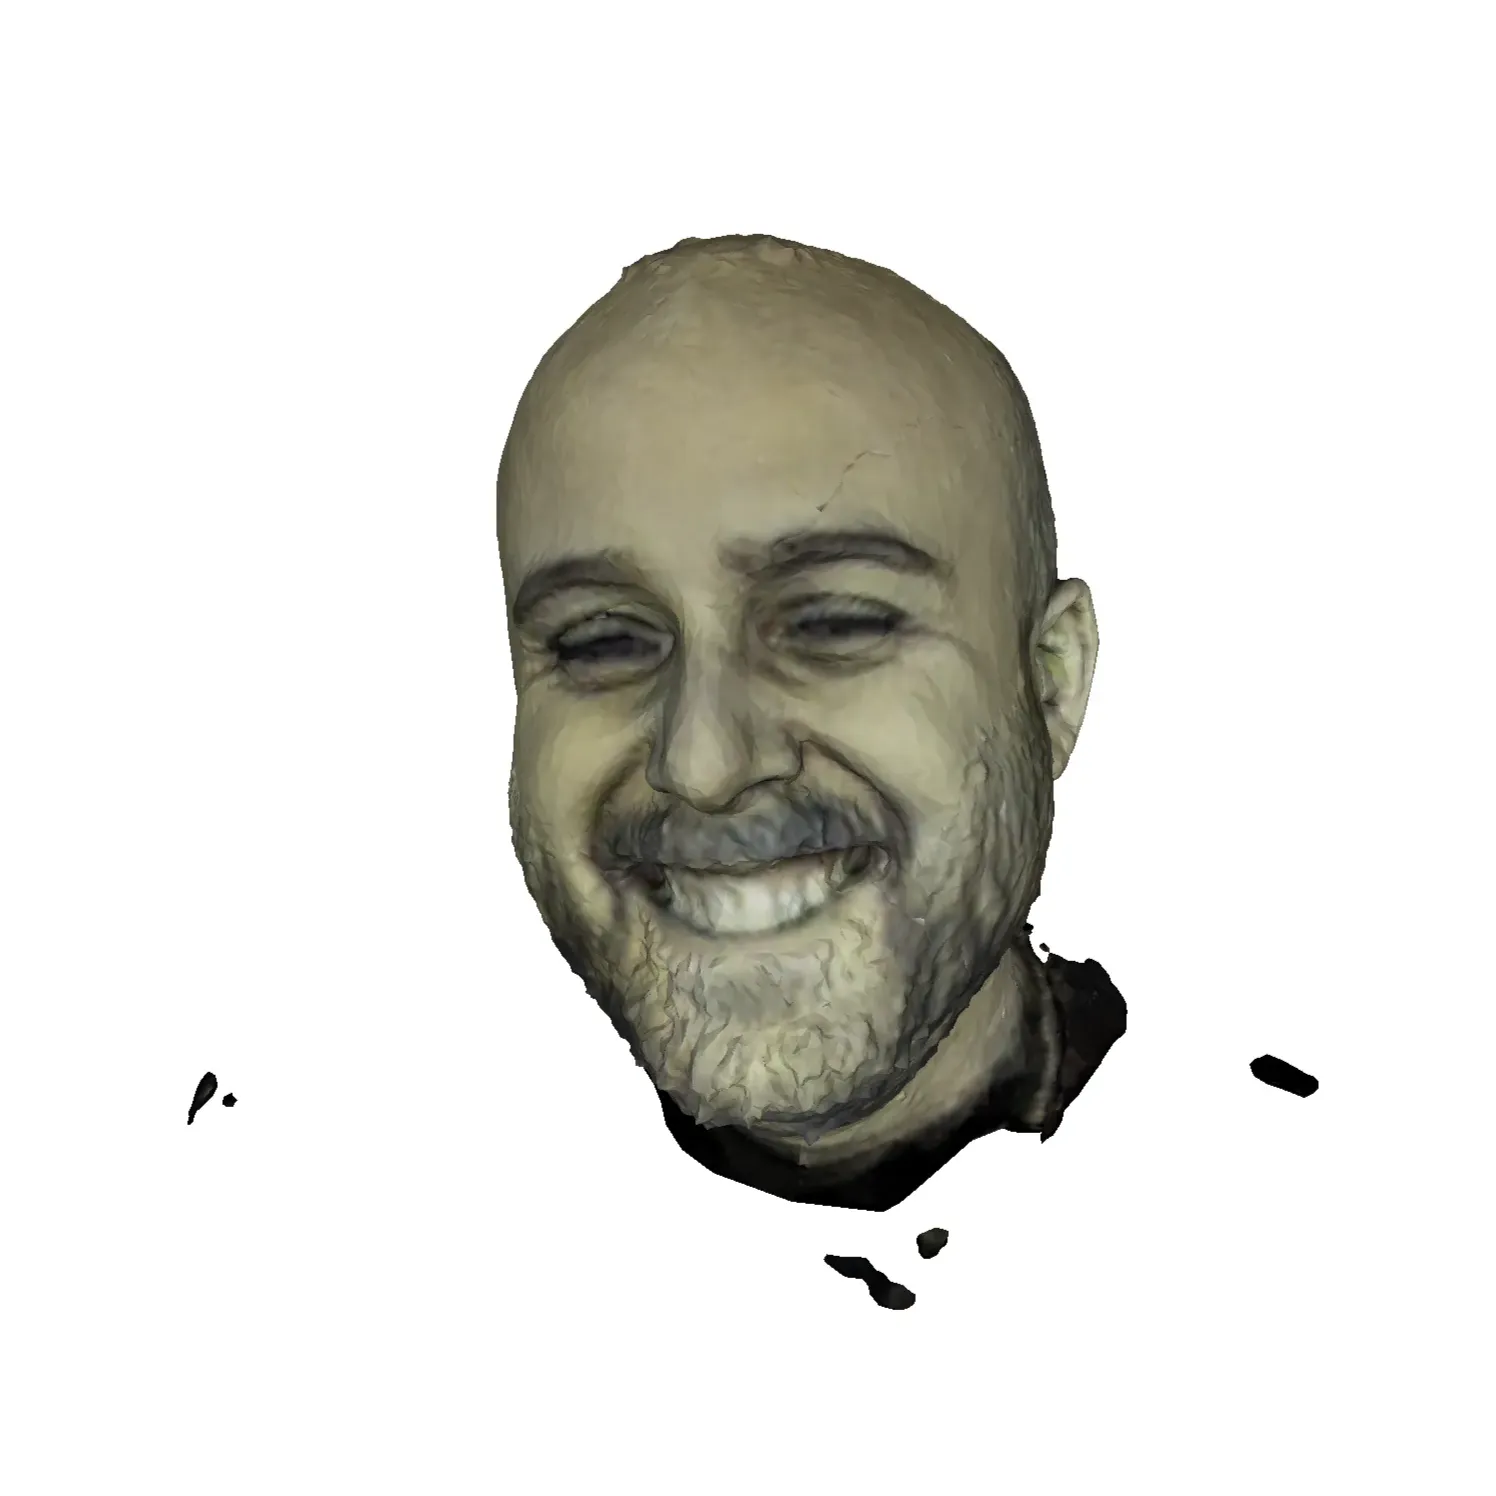
\includegraphics[width=\textwidth]{Figures/failed/stross/3d/snapshot10.png}
        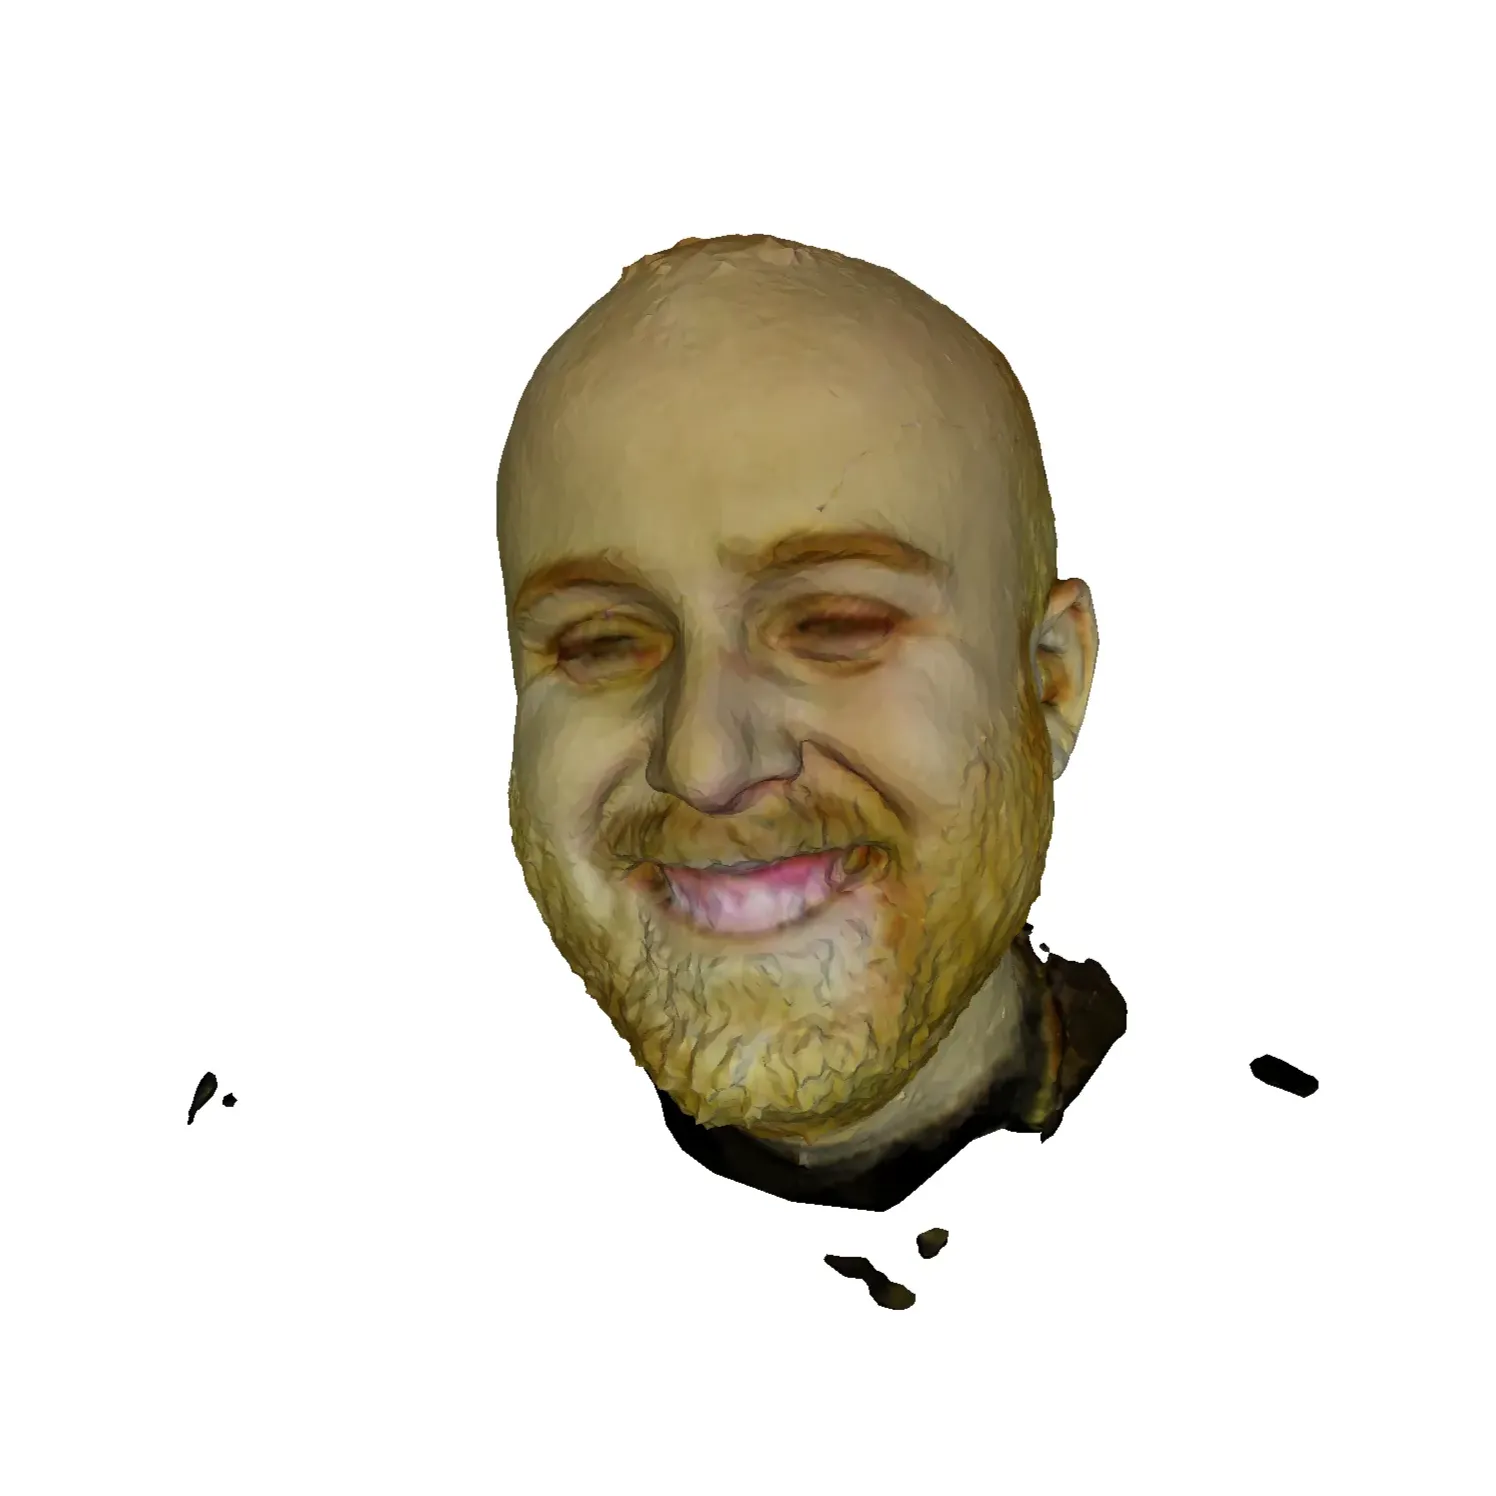
\includegraphics[width=\textwidth]{Figures/failed/stross/3d/snapshot11.png}
	\end{subfigure}
    \begin{subfigure}{0.18\linewidth}
        
\includegraphics[width=\textwidth]{Figures/failed/stross/3d/snapshot14.png}
        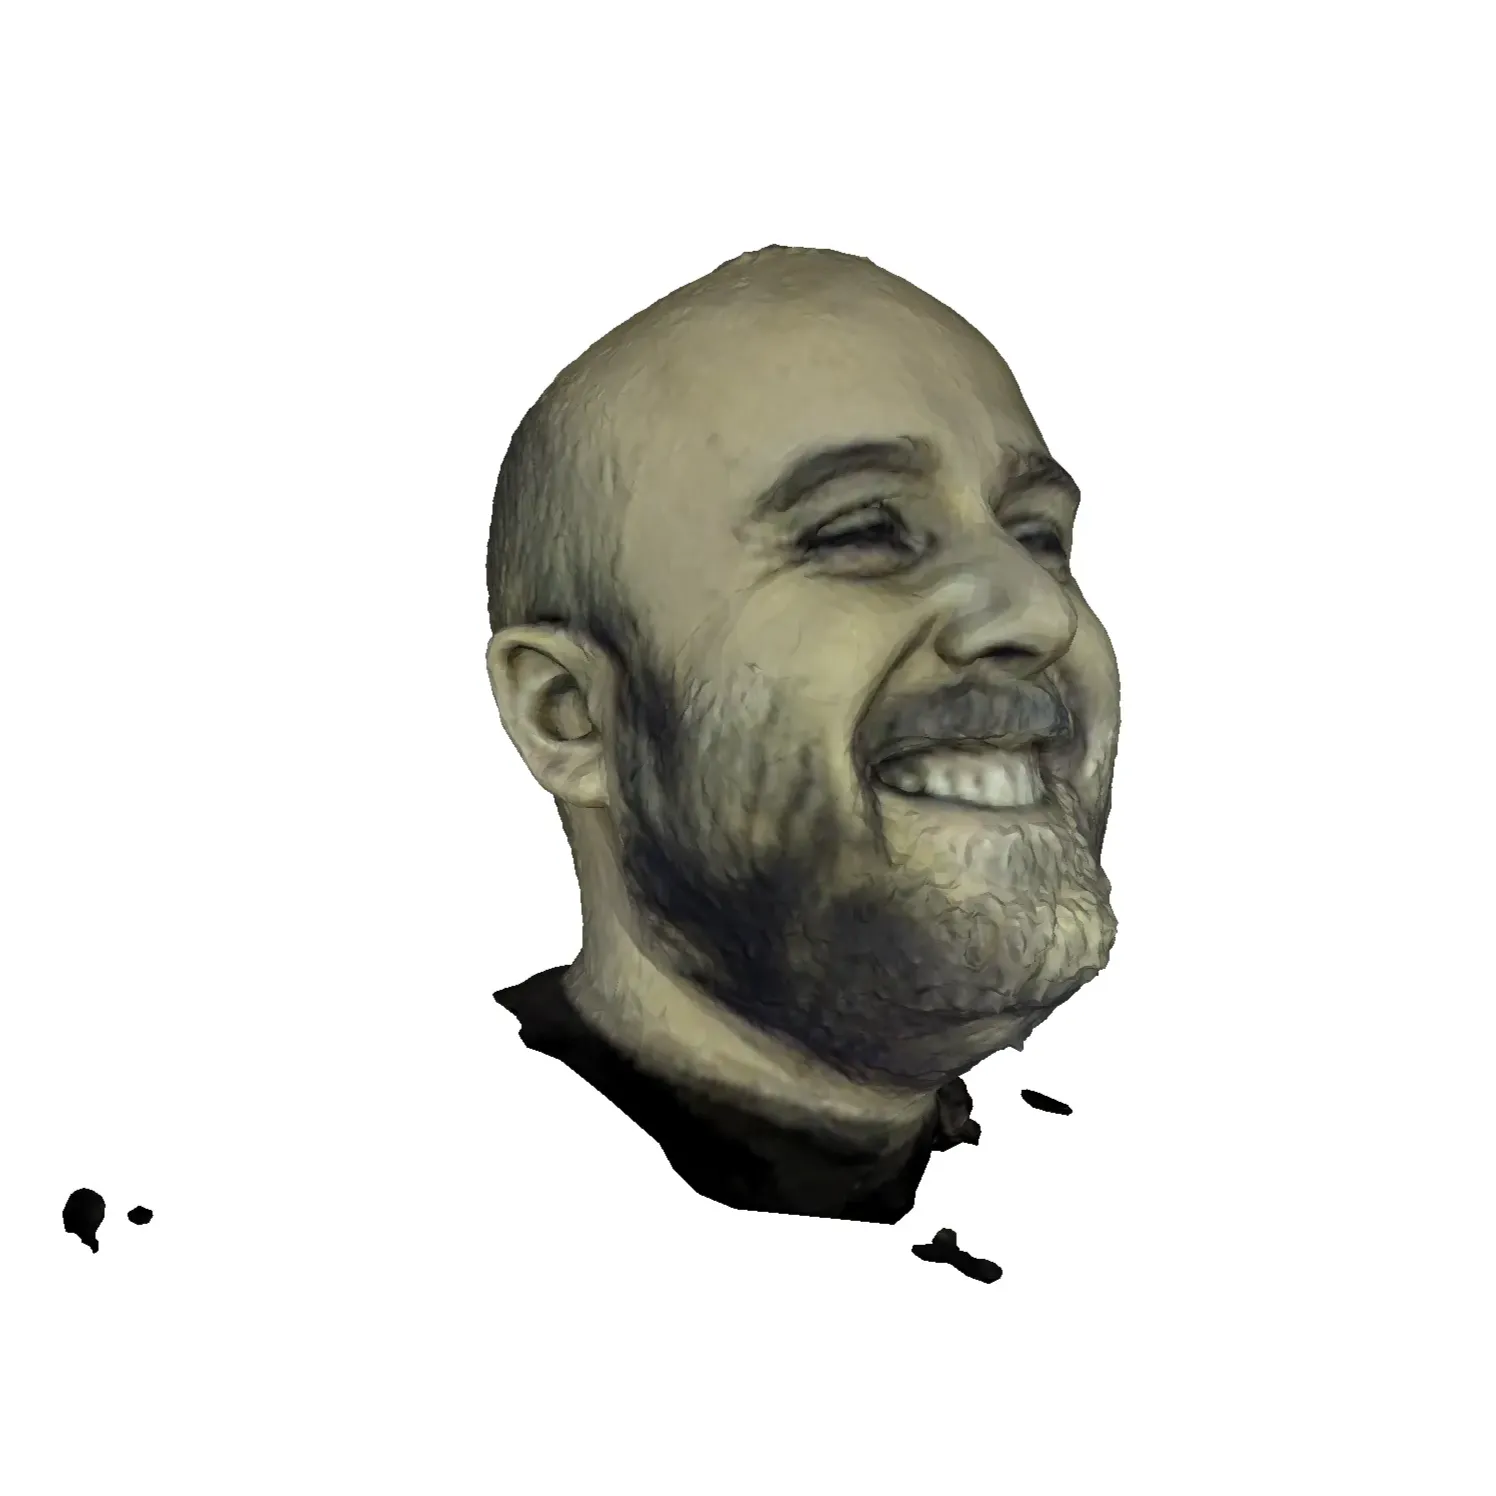
\includegraphics[width=\textwidth]{Figures/failed/stross/3d/snapshot13.png}
        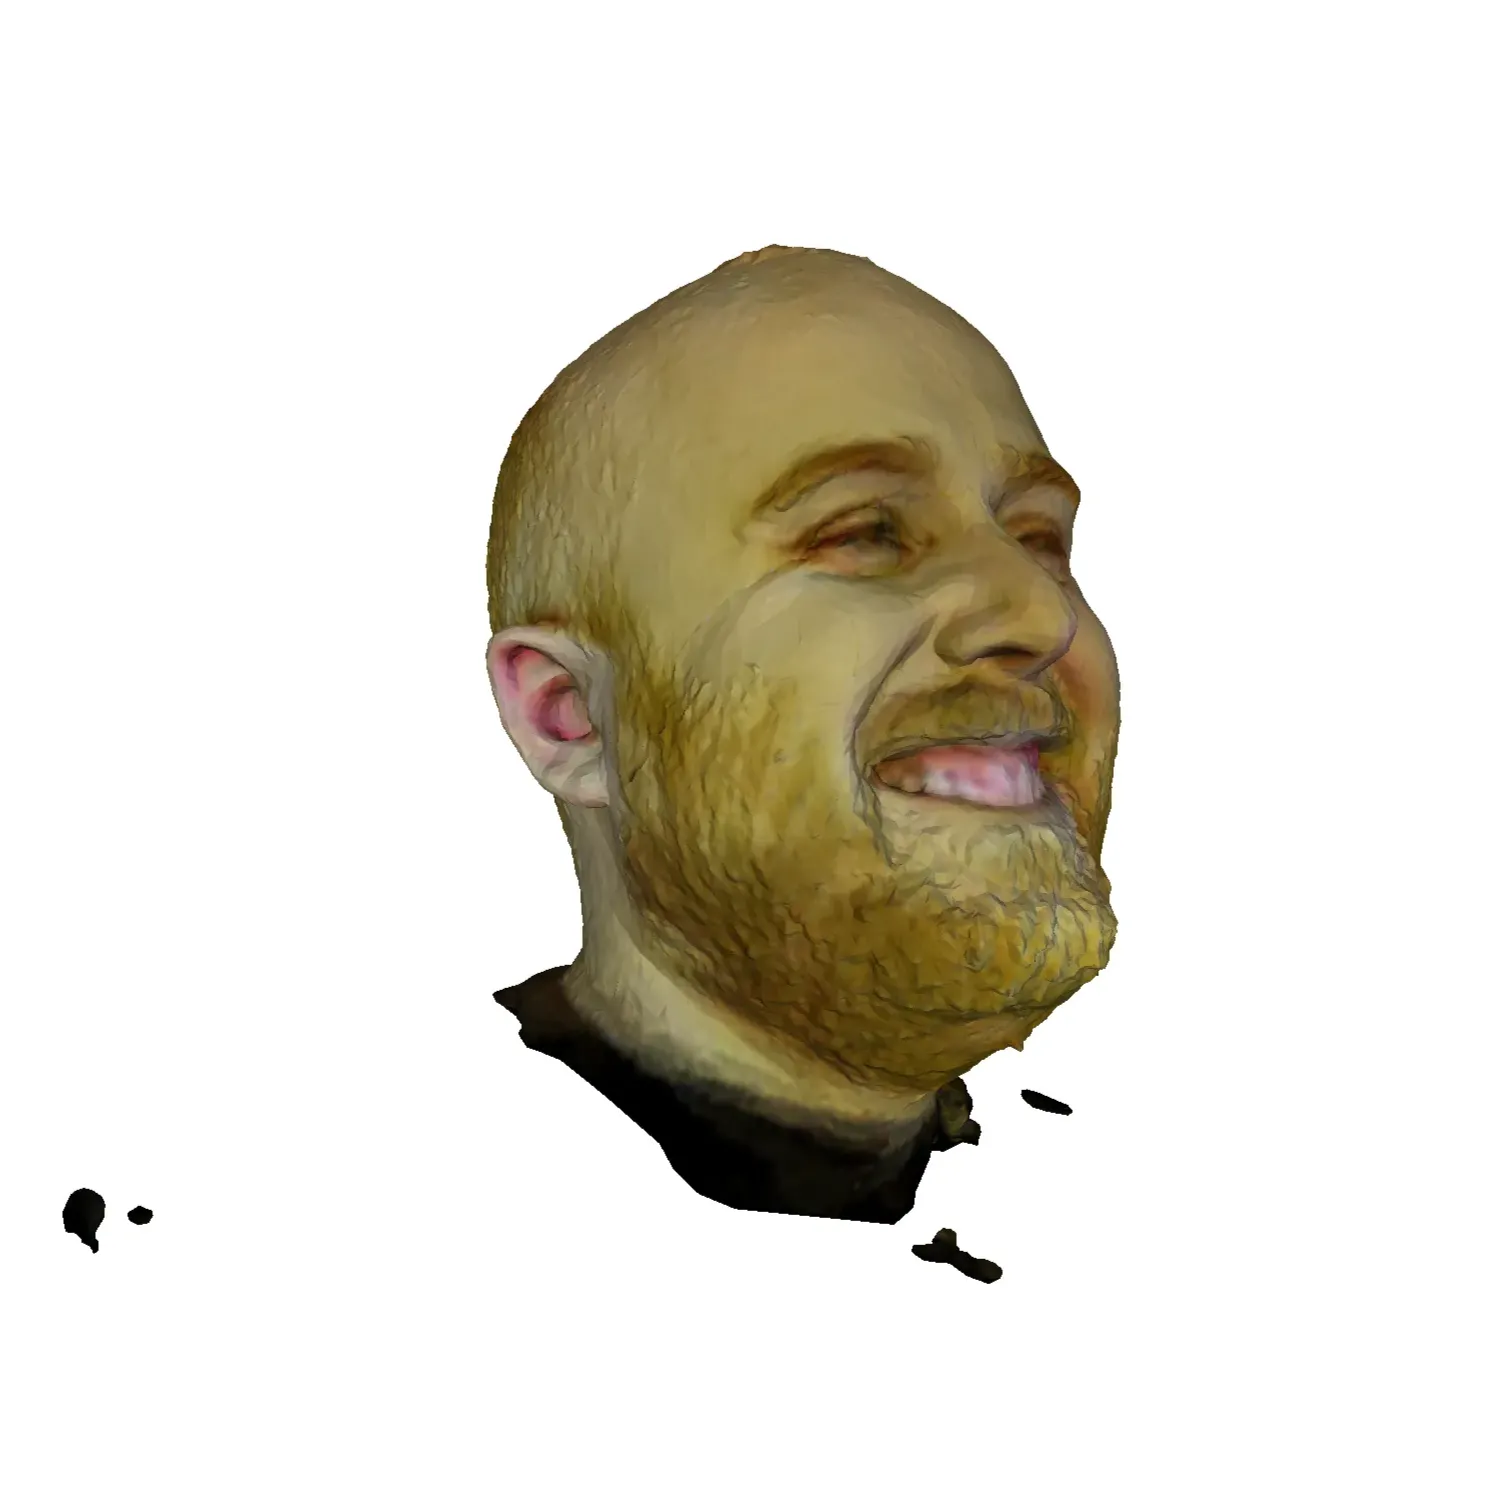
\includegraphics[width=\textwidth]{Figures/failed/stross/3d/snapshot12.png}
	\end{subfigure}
    \begin{subfigure}{0.18\linewidth}
        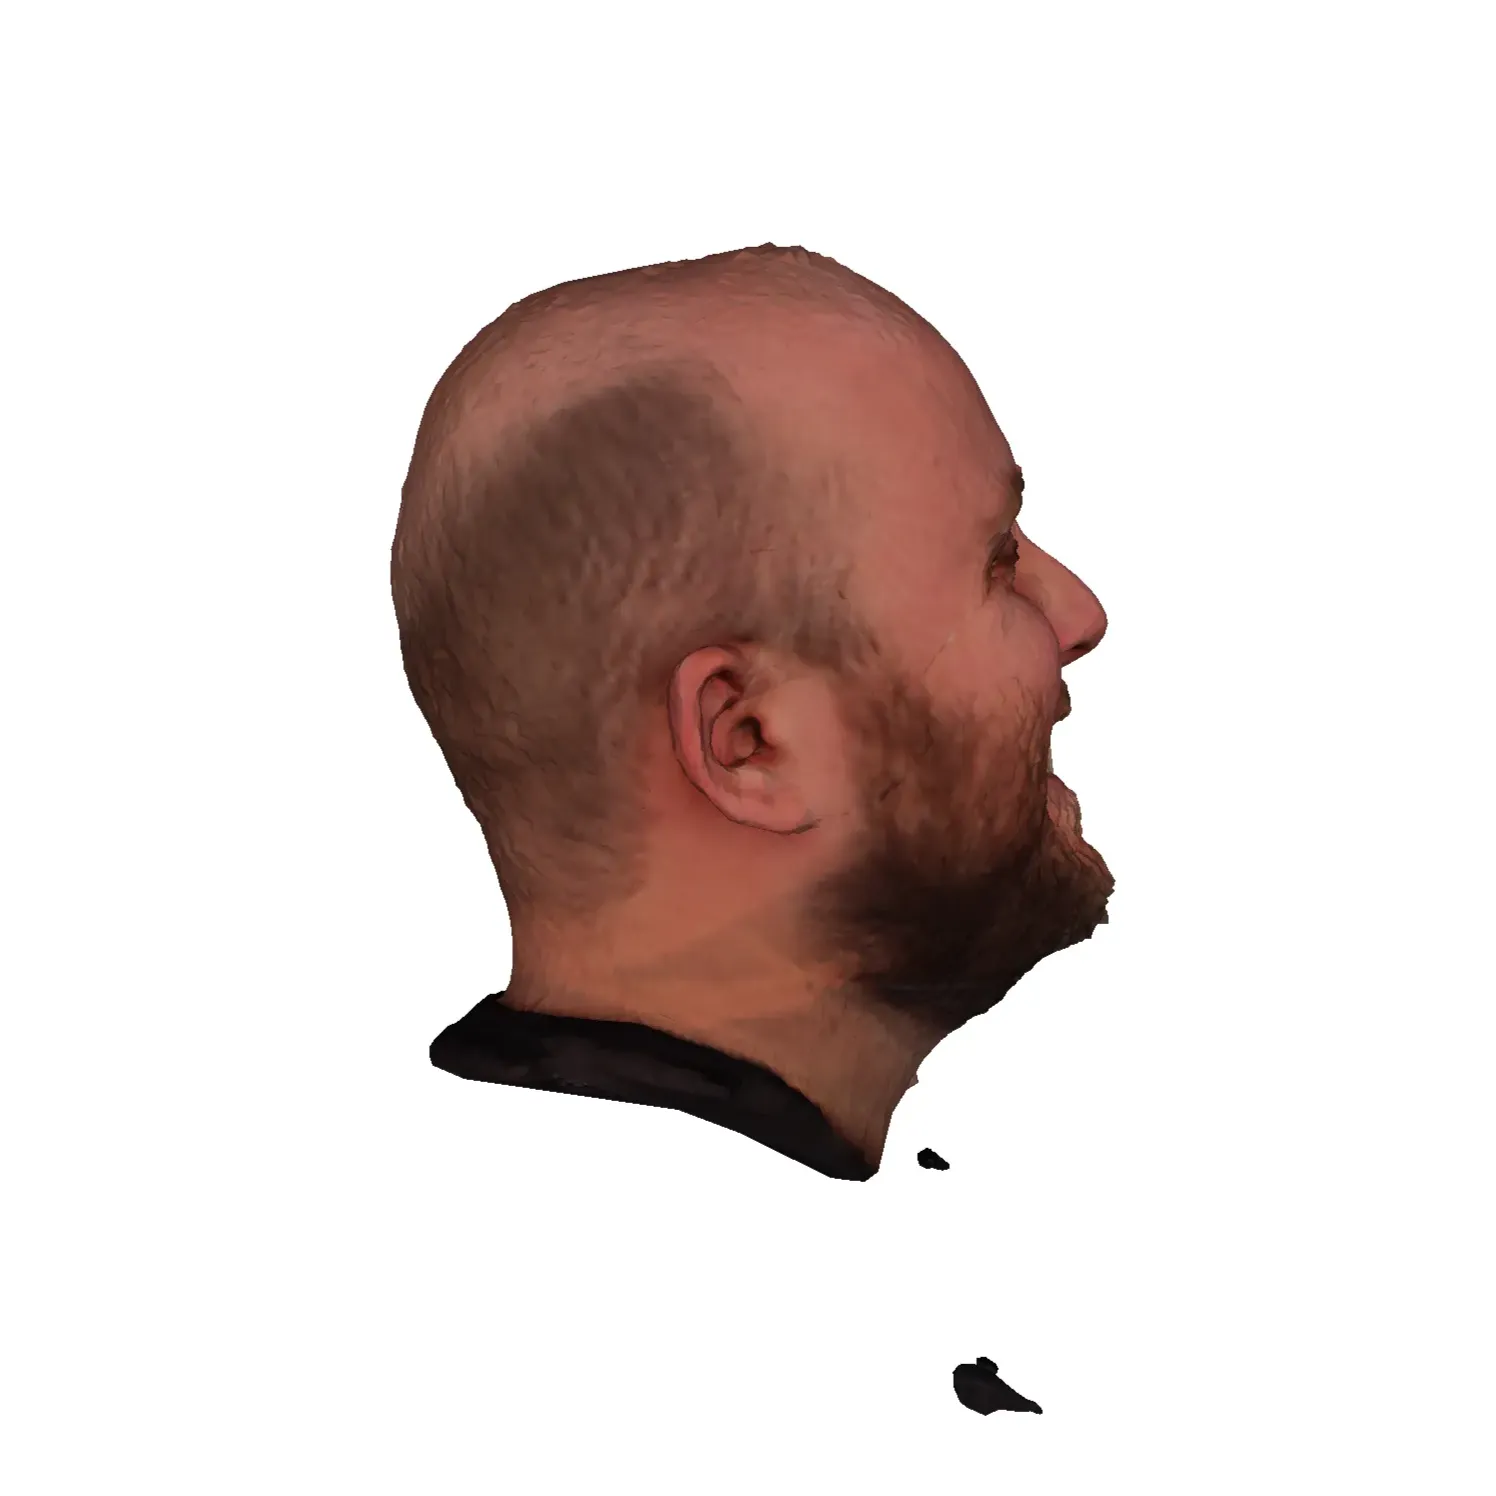
\includegraphics[width=\textwidth]{Figures/failed/stross/3d/snapshot15.png}
        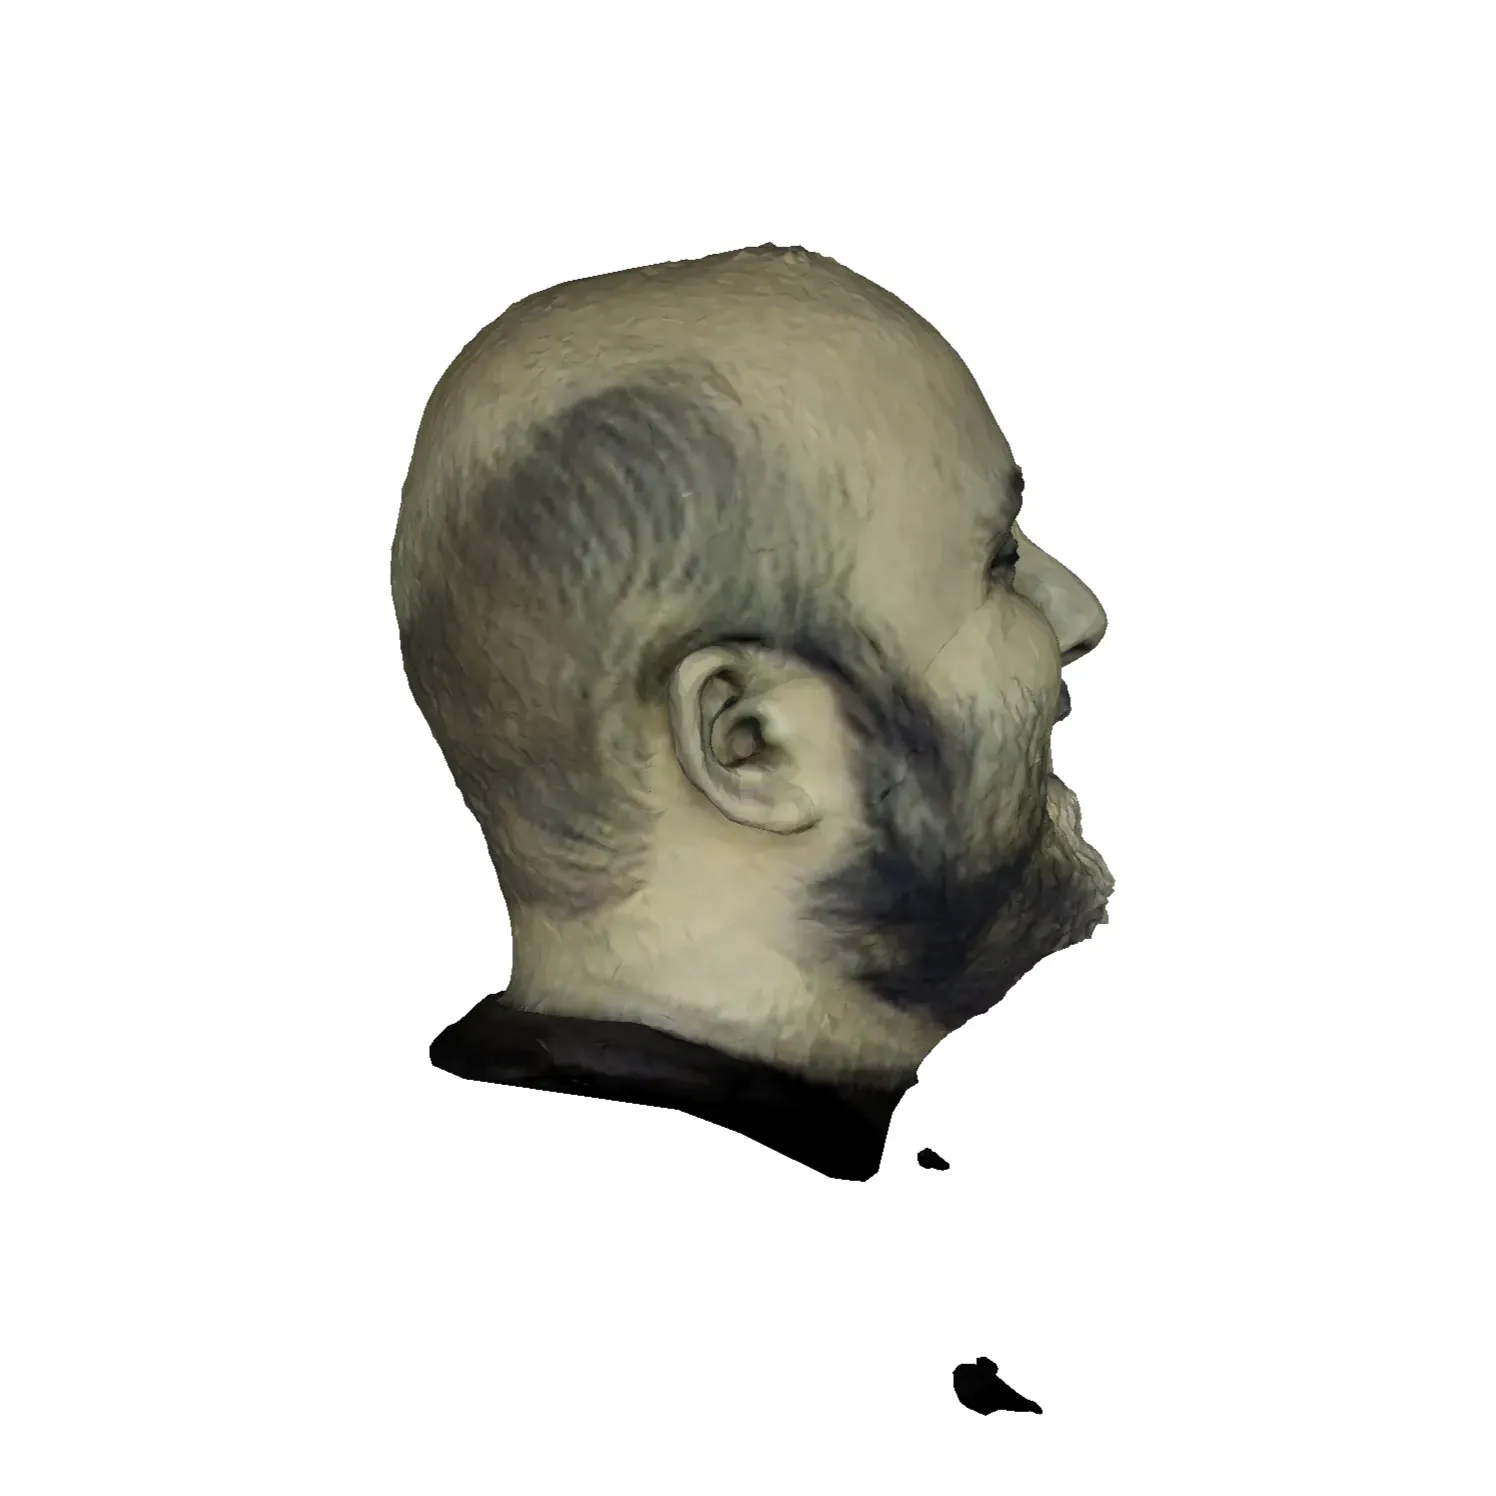
\includegraphics[width=\textwidth]{Figures/failed/stross/3d/snapshot16.png}
        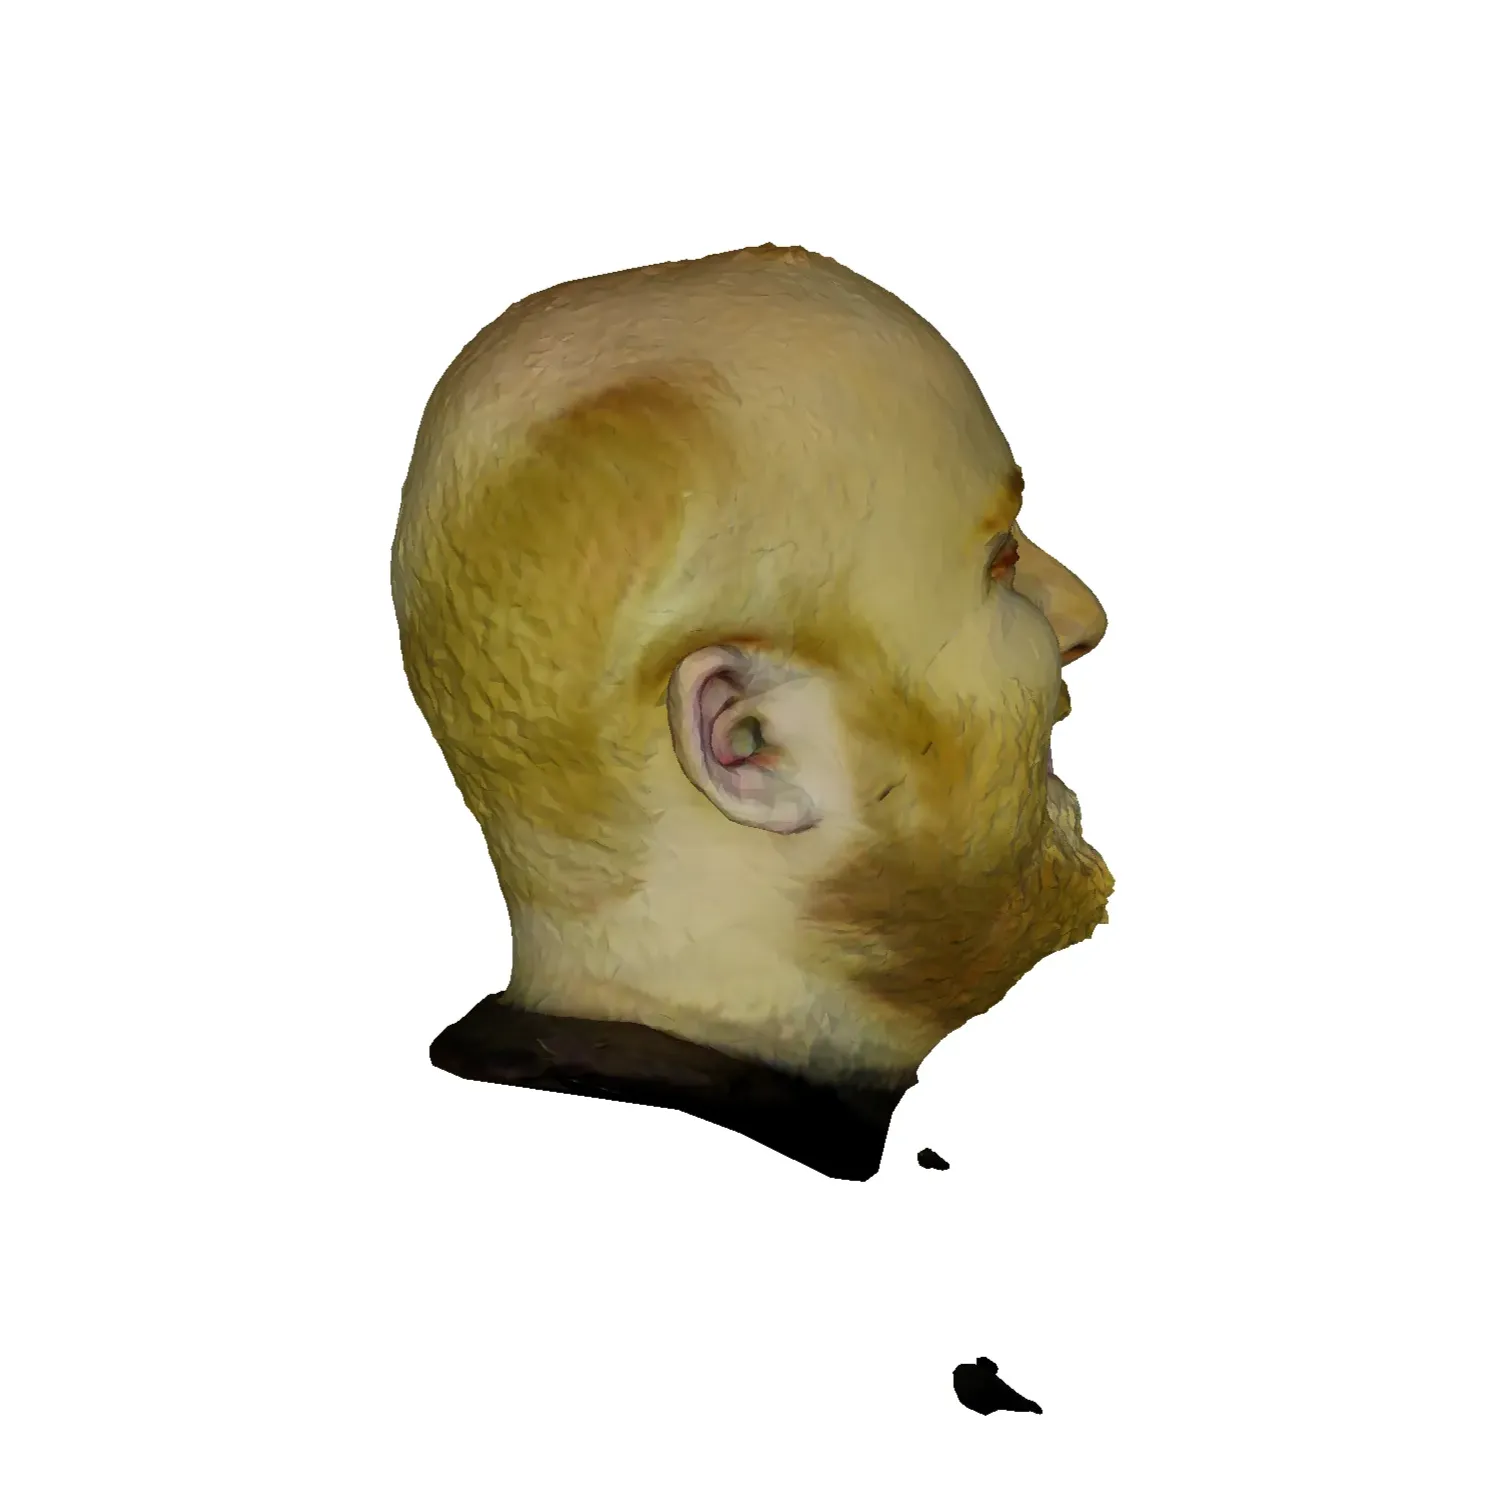
\includegraphics[width=\textwidth]{Figures/failed/stross/3d/snapshot17.png}
	\end{subfigure}
    \begin{subfigure}{0.18\linewidth}
        
\includegraphics[width=\textwidth]{Figures/failed/stross/3d/snapshot20.png}
        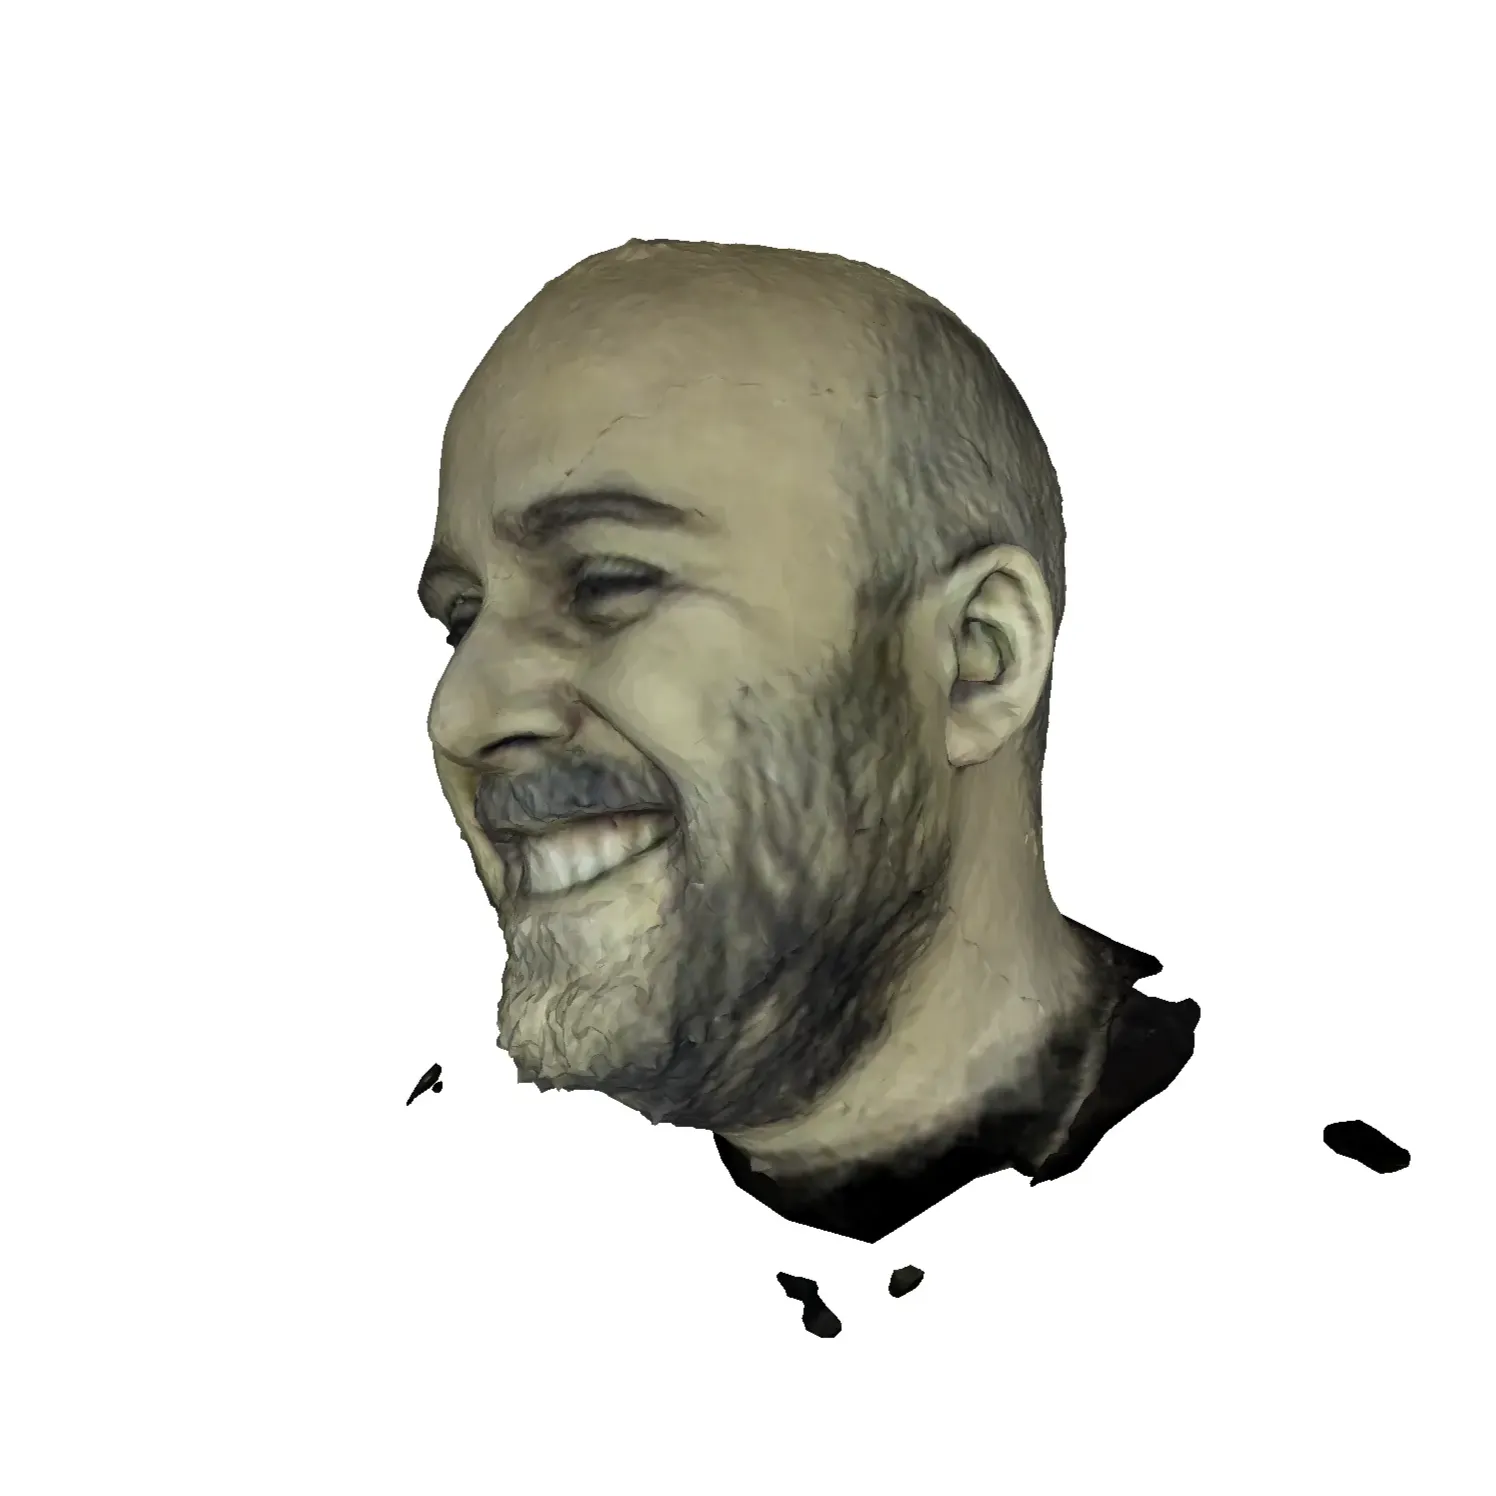
\includegraphics[width=\textwidth]{Figures/failed/stross/3d/snapshot19.png}
        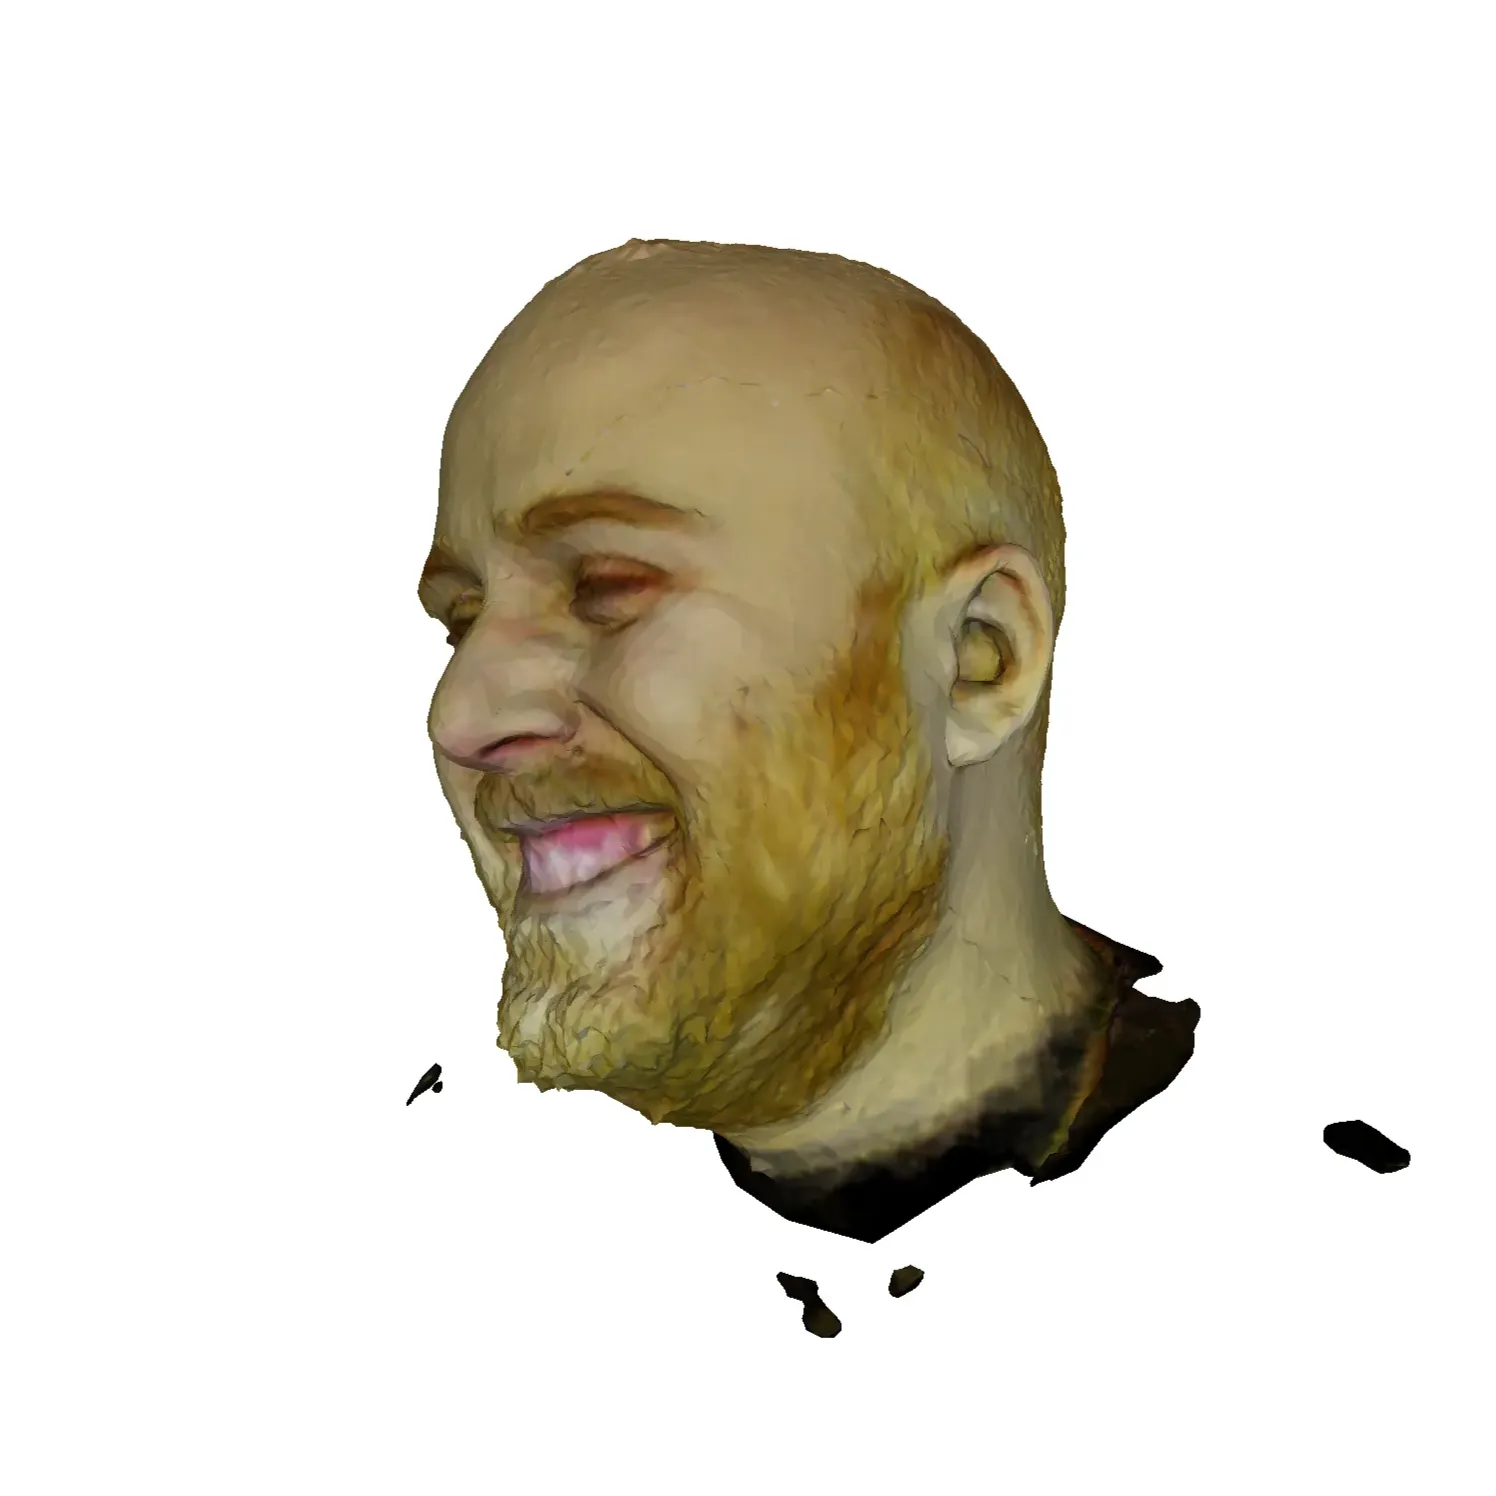
\includegraphics[width=\textwidth]{Figures/failed/stross/3d/snapshot18.png}
	\end{subfigure}
    \begin{subfigure}{0.18\linewidth}
        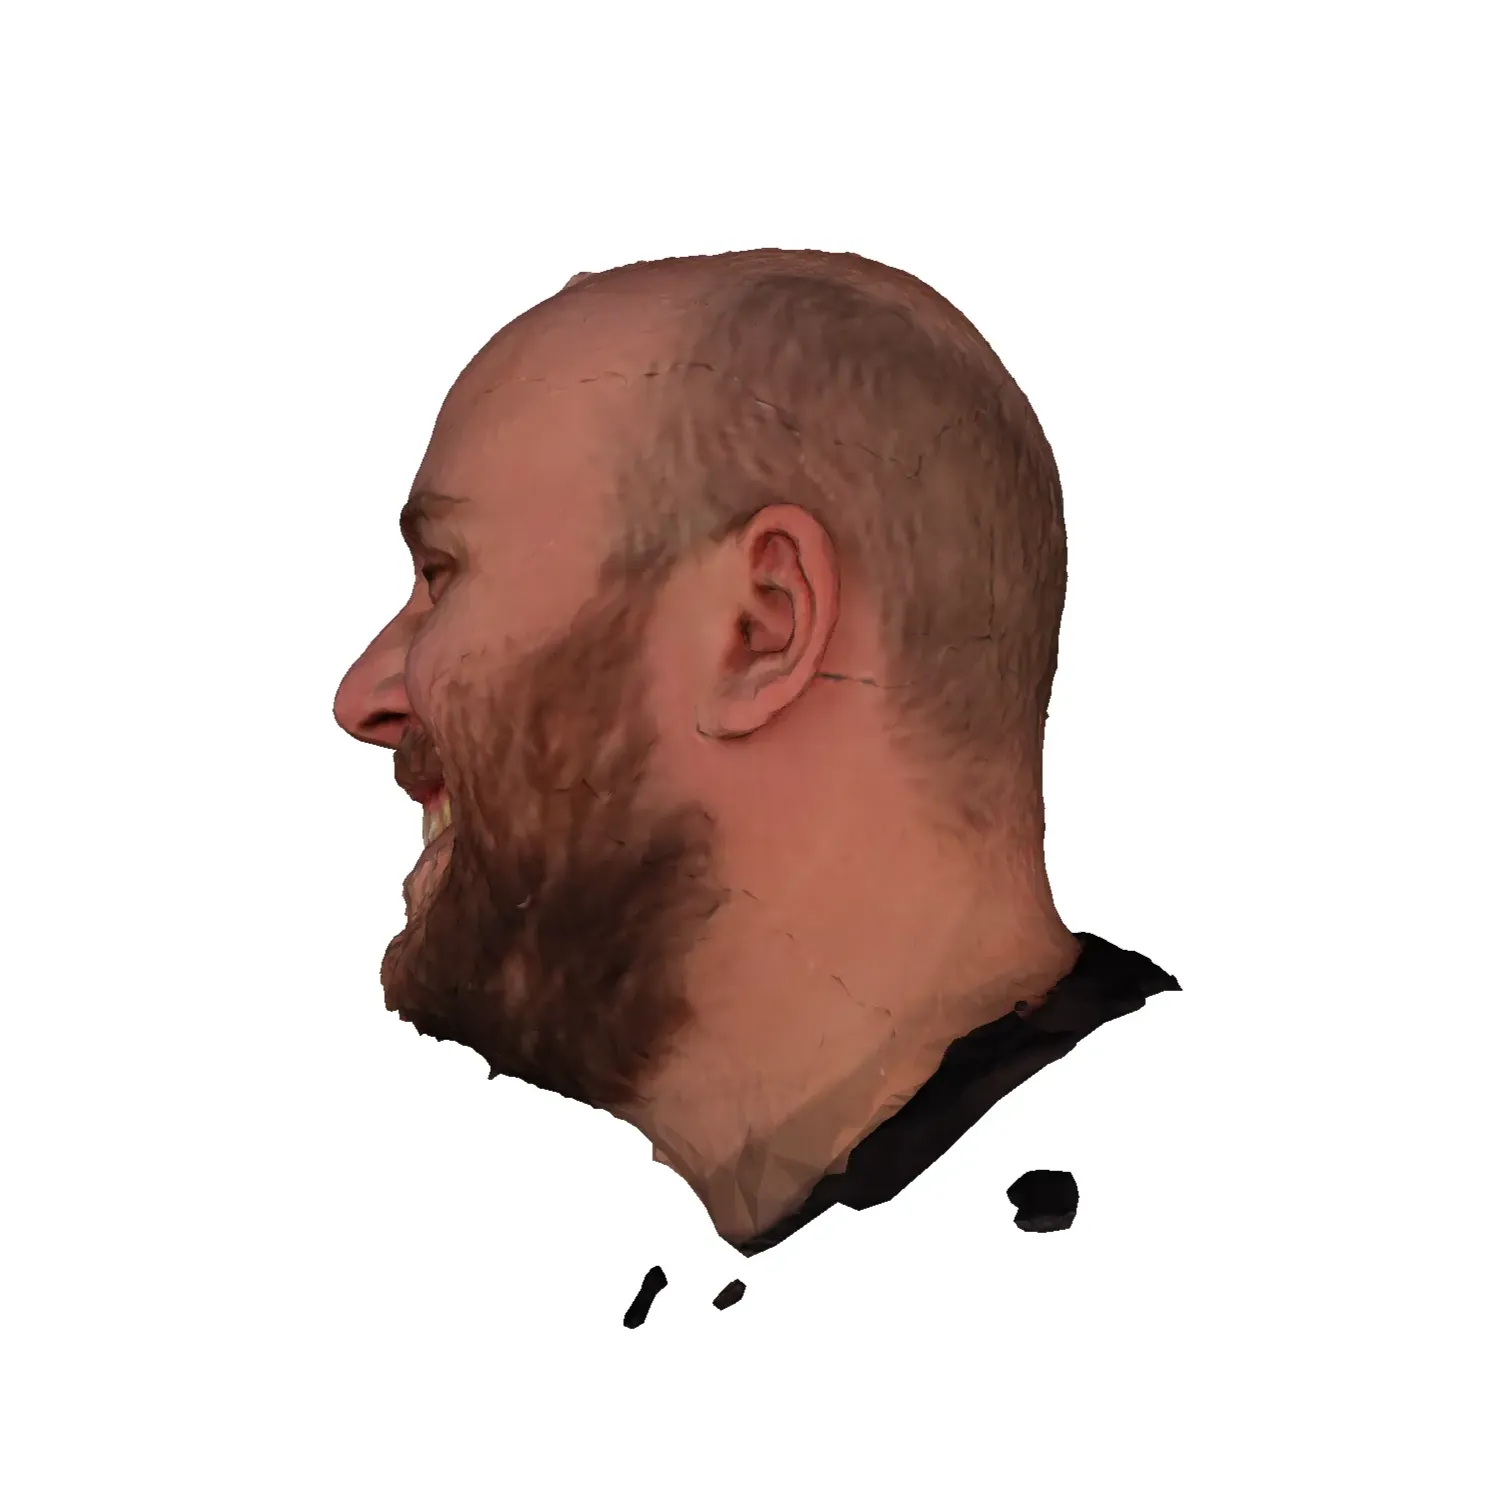
\includegraphics[width=\textwidth]{Figures/failed/stross/3d/snapshot21.png}
        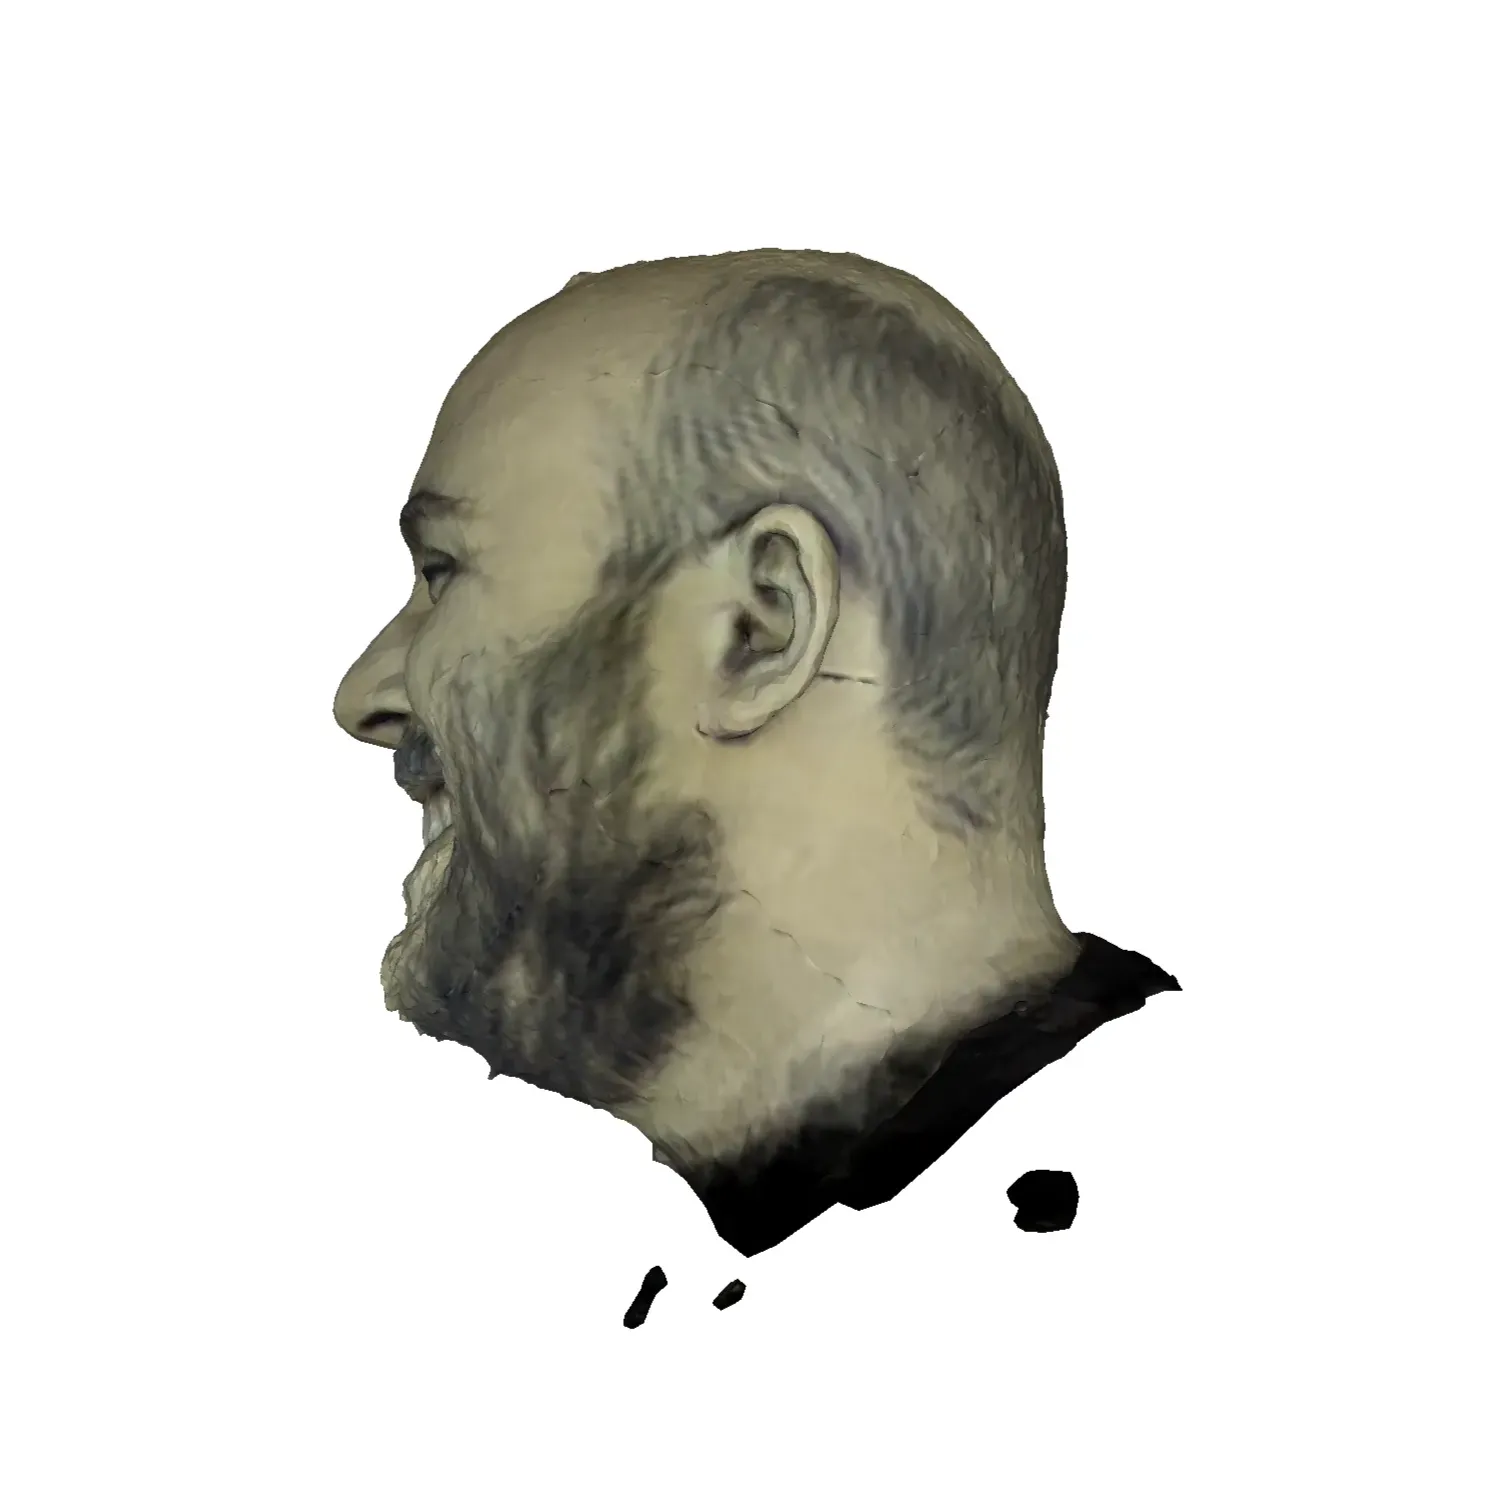
\includegraphics[width=\textwidth]{Figures/failed/stross/3d/snapshot22.png}
        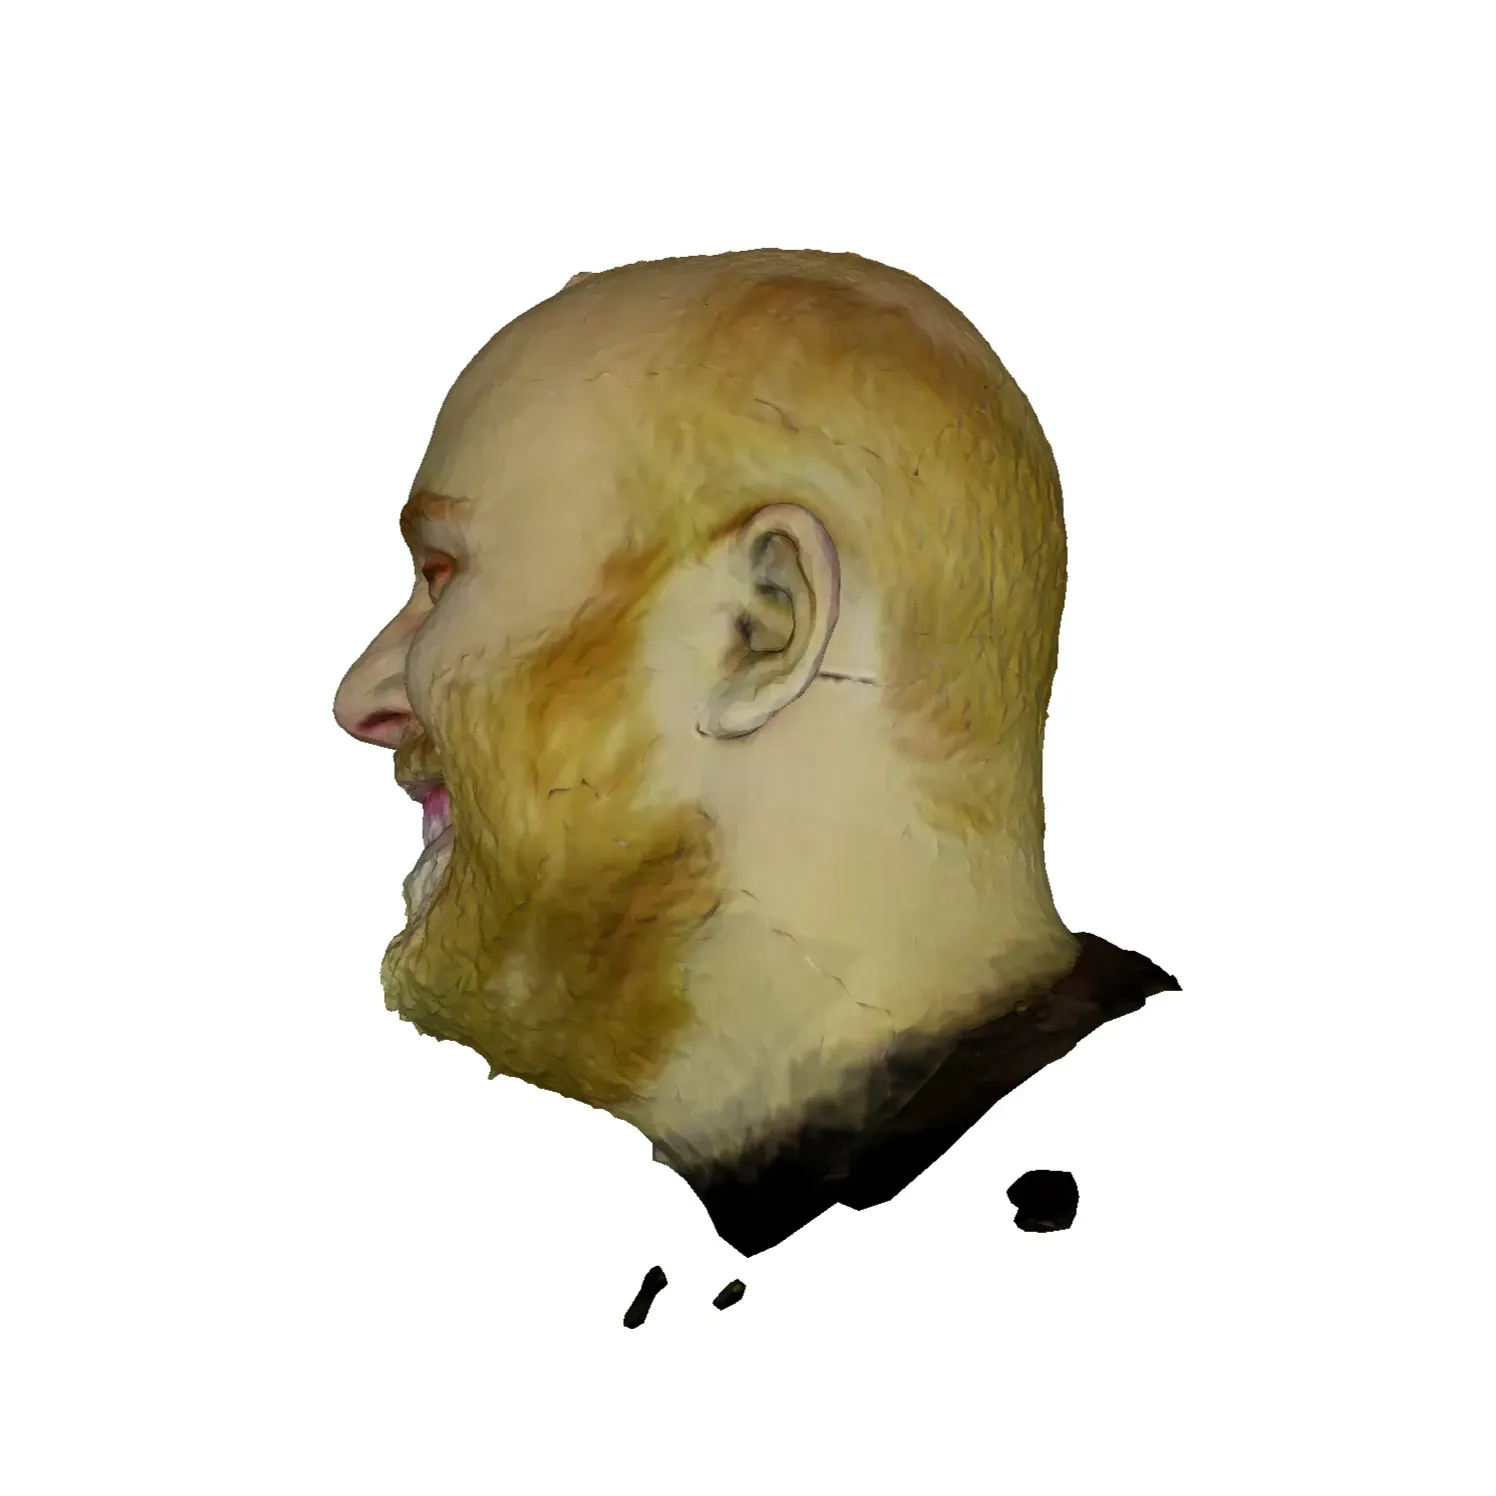
\includegraphics[width=\textwidth]{Figures/failed/stross/3d/snapshot23.png}
	\end{subfigure}
    \caption{Texture remapping using the stylized images from STROTSS pipeline on the canonical 3D avatar. The results show some success in transferring the texture from the style images to the 3D avatar and its multi-view consistency, but details are lost through texture blending.}
    \label{fig:stross_texture_fit}

\end{figure}


\section{InstructNerf2Nerf}
With \textit{InstructNerf2Nerf}, \textcite{Haque.2023} combine the flexibility of 3D representation in NeRF with the editing capabilities of InstructPix2Pix \citep{Brooks.2023}, addressing the multi-view inconsistency in InstructPix2Pix's editing process. Multi-view consistency in stylization is crucial in 3D style transfer to avoid undesired or unexpected deformations in the resulting 3D model. To leverage multi-view consistency, the authors propose an iterative dataset update during NeRF optimization. 
InstructNerf2Nerf takes a set of captured images of a real-world scene, corresponding camera parameters, and an initial NeRF reconstruction as inputs. It then generates a new NeRF scene conditioned by a text prompt through a series of latent diffusion steps using InstructPix2Pix. These diffusion steps are preconditioned with a constant latent representation of the unmodified images and the text prompt, creating a set of edited images. These edited images are used to update the NeRF dataset, generating an edited NeRF scene. This process is repeated until the scene converges to the desired, view-consistent style. The authors demonstrate that InstructNerf2Nerf can generate a stylized, text-prompt-conditioned 3D scene with view consistency within 10,000 iterations and three batches of diffusion steps per image. However, they acknowledge that the pipeline is computationally expensive and resource-intensive. Furthermore, NeRF inherently has slow rendering and production times, and achieving desired results often requires parameter adjustments and trial-and-error, consuming valuable time.


\section{InstructGS2GS and similar works}
As an alternative to InstructNerf2Nerf, \textcite{Vachha.2024} propose a more efficient and faster pipeline called InstructGS2GS. This pipeline employs a similar iterative dataset update approach but uses 3D Gaussian Splatting \citep{Kerbl.2023} instead of NeRF for 3D representation, sharing a similar dataset update logic. The authors show that InstructGS2GS can generate prompt-driven stylized 3D scenes more quickly and with fewer computational resources.

Several recent works \citep{Wang.2024, Wu.2024, Chen.2024, Chen.2023a, Jaganathan.2024} also use modified 2D Stable Diffusion pipelines for stylizing 2D images, each with distinct techniques to ensure view consistency and localized results in the 3D domain. \textcite{Wu.2024, Chen.2024} employ masking and attention mechanisms to localize stylization to specific image regions based on the text prompt. GaussCtrl, proposed by \textcite{Wu.2024}, uses ControlNet pipelines with depth-conditioned models to constrain stylization across multiple views. In contrast, \textcite{Chen.2024} compute epipolar lines for certain camera views and inject these features into InstructPix2Pix’s denoising network to ensure consistent stylization across views.

Two works named GaussianEditor (by \textcite{Wang.2024} and \textcite{Chen.2023a}) use InstructPix2Pix as their stylization backbone. \textcite{Wang.2024} proposes a mechanism that performs editing alignment from one view to its corresponding scene region using regional information from the prompt and the scene's semantic segmentation. \textcite{Chen.2023a} introduce Hierarchical Gaussian Splatting to refine 2D diffusion priors, ensuring consistent changes across views. \textcite{Jaganathan.2024} develop a texture and color editing framework that uses texture images as inputs, performs texture editing on sampled views, and applies changes to corresponding scene regions using image segmentation and mask matching, guided by a texture loss function to prevent quality degradation from texture mismatches.

This thesis aligns more closely with InstructGS2GS by \textcite{Vachha.2024}, given its straightforward approach and public accessibility. While the other works are more advanced and produce impressive results, they became accessible recently and require complex pipelines with high hardware and computational resource demands, unavailable during this thesis's writing. InstructGS2GS is built on Splatfacto pipelines in the Nerfstudio framework \citep{Tancik.2023}, with Gsplat \citep{Ye.2023} as its rasterizer, offering a more user-friendly and accessible framework for this task. Consequently, many methods in this thesis are derived from the aforementioned works, with some modifications based on experiments and insights from others, detailed in Section \ref{sec:stylization}.

\section{Evaluation Metrics for Stylization in 3D Gaussian Splatting}
In the aforementioned works, several metrics are used to quantitatively evaluate the stylized 3D scenes. The most common metric is the CLIP Text-Image Direction Similarity (CTIDS) \citep{Wang.2004, Chen.2024, Chen.2023a, Wu.2024}. Given a rendered view of the stylized scene and the text prompt, CTIDS measures the similarity between the prompt and the rendered image, evaluating if the scene is stylized as expected. However, it is unclear how each author applies this metric, and CTIDS does not consider the consistency of edits across multiple viewpoints. Additionally, \textcite{Wu.2024} note that CTIDS does not necessarily reflect editing quality.

This thesis draws inspiration from \textcite{Liu.2024} in StyleGaussian, where one stylized view is warped to another using optical flow and softmax splatting, creating warped and target image pairs. RMSE and LPIPS scores are computed in the masked overlapping areas to measure stylization consistency, similar to the technique used by \textcite{Mu.2021} and \textcite{Huang.2021}. Although user studies \citep{Jaganathan.2024, Wang.2004, Chen.2024, Chen.2023a, Wu.2024} are common quantitative evaluation methods, this thesis does not include them due to the use of human models and identity protection concerns. Instead, the evaluation is conducted qualitatively using the aforementioned metrics and techniques, described in Chapter \ref{sec:metric}.